\chapter{Proposed Algorithms}
\section{Multi-target Search} 
\label{algo}
In this section, we discuss how to effectively adapt Polyanya for OkNN settings where there are multiple
candidate targets (cf. just one). Since Polyanya instantiates A* search, and since that algorithm is itself a special case of Dijkstra's well known technique, there exists a simple modification at hand: we can simply remove the influence of the cost-to-go heuristic and allow the search to continue until it has expanded the $k^{th}$ target. All other aspects of the algorithm, including termination\footnote{There are two cases to consider depending on whether the query and target points are in the same polygon or in different polygons. Both are described in~\cite{cuicompromise}}, remain unchanged.

The version of Polyanya we have just described is unlikely to be efficient. Without a heuristic function for
guidance nodes can only be prioritised by the $g$-value of their root point, 
which is settled at the time of expansion.
However, the $g$-value does not reflect the distance between the root and its corresponding interval. 
For example, in Figure~\ref{suc}, all observable successors would have the same expansion priority.
Thus we may expand many nodes, all equally promising but having distant intervals, and all before reaching a nearby target node with a slightly higher $g$-value.
To deal with this problem we develop two online heuristics which can be fruitfully applied to OkNN:
\begin{itemize}
    \item The Interval Heuristic, which prioritises nodes using the closest point 
    from its associated interval. 
    \item The Target Heuristic, which relies on a Euclidean nearest-neighbour estimator to 
    provide a target dynamically at the time of expansion. 
\end{itemize}
\noindent
Each of these heuristics is applied in the usual way compute a final expansion priority: 
$f(n) = g(n) + h(n)$ where $g(n)$ is the (known) distance from the query point to the root, 
and $h(n)$ is a lower-bound on the distance to the next target. 
In the remainder of this section we explore these ideas in turn.
In the experimental section thereafter we will also consider a third, even simpler strategy for
multi-target search: 
repeatedly call an unmodified point-to-point Polyanya search, from the query point and to 
each target. In a perhaps surprising result, we will show that each of these three alternatives 
yields state of the art performance in certain contexts.

\subsection{Interval Heuristic}
\label{sec::ih}

In some OkNN settings targets are myriad and one simply requires a fast algorithm to explore the local area. This approach is in contrast to more sophisticated methods which apply spatial reasoning
to prune the set of candidates. 
The idea we introduce for such settings is simple and can be formalised as follows:


\begin{definition}
  Given search node $(I, r)$, the Interval Heuristic computes a value $h_i(I, r)$ which
  is the minimal Euclidean distance from the root $r$ to the segment $I$.
\end{definition}

Applying the Interval Heuristic $h_i$ requires solving a simple geometric problem: finding the
closest point on a line. The operation has low constant time complexity and we apply
standard techniques. Algorithm~\ref{intervalsrc} shows an example.

\begin{algorithm}
  \input{./code/interval.pseudo}
  \caption{Interval Heuristic Search}
  \label{intervalsrc}
\end{algorithm}

\begin{theorem}{\textbf{(admissibility)}:}\label{nodesc}
  The $\textit{f-value}$ of successor node is not less than the $\textit{f-value}$ of the parent
  search node.
\end{theorem}

\begin{proof}
  Using the interval heuristic, when the successor is a search node, its \textit{f-value}
  can be interpreted as a lower-bound of the length of path from
  $s$ to any point on the segment $I$ through root $r$, and since it is generated by pushing
  away from the parent search node, its \textit{f-value} is larger than \textit{f-value}
  of the parent search node. If successor is a target node, the \textit{f-value} is the the length
  of the corresponding path and not less than the parent search node (the two values are equal 
  when the target is on the segment $I$).%$\square$
\end{proof}

\begin{corollary}
  Expanding a target node corresponds to finding a shortest path.
\end{corollary}

\begin{proof}
  As per Theorem~\ref{nodesc}, when a final node is expanded there exists
  no remaining candidate on the open list which can reach the node with a smaller $f$-value.
\end{proof}

\subsection{Target Heuristic} 
\label{theuristic}
In some OkNN settings the set of targets are few (i.e. sparse) and without a reasonable 
heuristic guide it is possible to perform many redundant expansions in areas where no nearest
neighbour can exist. In such cases more sophisticated spatial reasoning can help to prune the
set of nearest neighbours and guide the search. The idea we introduce for such settings can
be formalised as follows:


\begin{definition}\label{close}
  The minimum distance to the closest target $t$ of a search node $n=(I, r)$ at least equal to 
  $h$(n, t) =  $\mathbf{min}\{d_e(n, i) | i \in T\}$, where $d_e$ is the Euclidean metric.
\end{definition}

The definition says that, when expanding a node, we can always use as a guide the minimum Euclidean distance, from the current node to any of the possible candidate target points. 
We implement this idea as follows. 
First, we divide the space around the current interval $I$ into four regions, as shown in Figure~\ref{fa}.
Then, following the example, we may reason as follows:
\begin{figure}[ht]
  \centering
  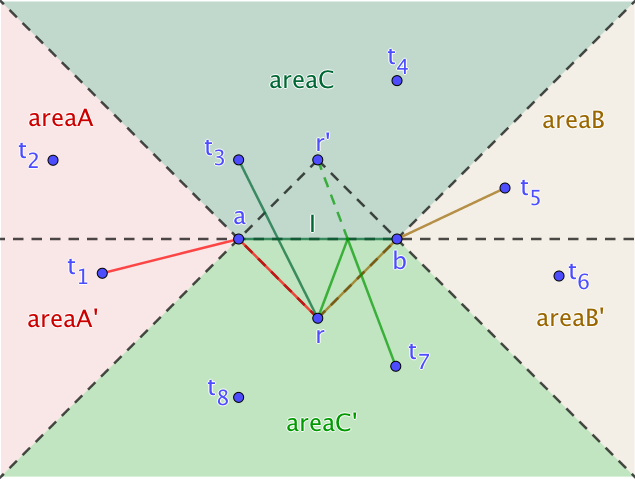
\includegraphics[width=\linewidth]{pic/heuristic.png}
  \caption{}
  \label{fa}
\end{figure}


\begin{itemize}
  \item Suppose the next nearest target $t$ is in $areaA$ (equiv. $areaB$). Then the optimal path must pass through the point $a$ (equiv. $b$) so the minimum $h$-value can be computed as: $\mathbf{min}\{d_e(r, a) + d_e(t, a)\}$ such that $t$ in $areaA$ (equiv. $areaB$).
  \item Alternatively, suppose the next nearest target $t$ is instead in $areaC$. Then the optimal path must pass through a point $p$ in the open  interval $(a, b)$. So the minimum $h$-value can be computed by minimising across all target points in $areaC$. A similar argument applies to a next nearest neighbour in $areaC'$ and we can apply a similar strategy, but only after mirroring the root point $r$ through the interval. This operation is in contrast to the admissible $f$-value estimate used by Polyanya in the point-to-point setting, which mirrors the target through the interval.
\end{itemize}

\noindent
Identifying the candidate target with minimum $h$-value in each of the four cases can be improved,
from a linear-time operation to one that runs in logarithmic time, by storing all of the targets in a spatial data structure such as\textit{R*-Tree}~\cite{beckmann1990r}. Thus we may compute a lower-bound
estimate to the next nearest neighbour by minimising over four candidates returned by the $R*$-tree instead of evaluating all possible target points.

\subsection{Further Refinements}
We may notice that the Target Heuristic described thus far is potentially costly, requiring 
four logarithmic operations as compared to one constant time operation in the point-to-point case.
To mitigate this we could call the function less often. For example we can assign the nearest-neighbour candidate computed at the parent node to each successor. We decide when to switch back to the Target heuristic using the point-to-point estimator: if the value is different from parent to child we need
to compute a new next nearest neighbour candidate. We call this strategy \textit{lazy compute}
and apply it throughout our experiments. We find it reduces total running time by approximately
20\%.

\begin{lemma}\label{lazy-compute}
  Given search node $n=(I,r)$, its successor $n'=(I', r')$, and a target $t$ that minimises Euclidean distance to $n$ from among all possible candidates. Further suppose $h_e$(n, t) = $h_e$(n', t), where $h_e$ is the Polyanya point-to-point estimator. Then $t$ is also a target that minimises Euclidean distance to $n'$ among all possible candidates.
\end{lemma}

\begin{proof}
  If there is $t'$ closer to $n'$ than $t$, then $h_e(n', t') <
  h_e(n', t) = h_e(n, t)$, and because of Lemma~\ref{nodesc},
  $h_e(n, t') <= h_e(n', t')$, so,
  $t$ can't be the closest target of $n$, which is conflict with assumption. Thus, such $t'$
  doesn't exist.
  %$\square$
\end{proof}

Now, each search node has a target, and the search behavior should be broadly similar to 
the point-to-point setting.
But there is one significant difference: when a nearest neighbor $t$ has been found, $t$ should
no longer influence the search process. Thus, we need to remove $t$ from search space and 
re-assign (i.e. update) all search nodes in the queue which use $t$ as their closest target. 
To avoid exploring the entire queue we propose instead the following simple strategy: 
when such a node is dequeud from the open list, we apply $h_t$ to compute a new target
and we push the node back onto open all without generating any successors. 
We call this \textit{lazy reassign}.

\begin{lemma}\label{lazy-reassign}
  Let's call these search nodes who need reassignment \textbf{pseudo nodes}, and others
  \textbf{real nodes}. \textbf{Lazy reassign} never changes the relative order of real
  nodes in queue.
\end{lemma}

\begin{proof}
  Let $n_1, n_2$ be any pair of real nodes, and $s$ be any pseudo node.  After the reassignment,
  if $s$ become neither $n_1$ nor $n_2$, then inserting a third party search node has nothing to do with the relative order of $n_1$
  and $n_2$; otherwise, without the loss of generality, assume $s$ becomes $n_1$. If the relative
  order of them is $<n_2, s>$, then $f(n_2) <= f(s)$, and
  because of the definition~\ref{close}, we have $f(s) <= f(n_1)$, so
  relative order of $n_1, n_2$ doesn't change. Alternatively, if the relative order is $<s, n_2>$, then $n_1$  will be push to queue before $n_2$ pop out, so the relative order of $n_1, n_2$ doesn't
  change as well.%$\square$
\end{proof}

In Algorithm~\ref{hsearch}, we arrive at last at the final form of Polyanya OkNN. The algorithm
accepts either $h_i$ and $h_t$ as a heuristic function and has, in both cases, the same high level steps.

\begin{algorithm}[t]
  \input{./code/hsearch.pseudo}
  \caption{Target Heuristic Search}
  \label{hsearch}
\end{algorithm}


